% fig-stone-zoom.tex
% "The Stone's Secret: Macro Stillness, Atomic Motion"
% Standalone TikZ figure — Ch. III
\documentclass[tikz,border=6mm]{standalone}
\usepackage{tikz}
\usepackage{xcolor}
\usetikzlibrary{arrows.meta,calc,decorations.pathmorphing,decorations.markings,shapes.geometric,positioning,backgrounds,fit,shadings,patterns}
\definecolor{substblue}{RGB}{70,130,180}
\definecolor{procamber}{RGB}{180,110,30}
\definecolor{feltgreen}{RGB}{0,110,55}
\definecolor{bgcream}{RGB}{252,248,240}
\definecolor{atomblue}{RGB}{100,160,210}
\definecolor{emphred}{RGB}{160,40,40}
\definecolor{panelborder}{RGB}{180,170,155}

\begin{document}
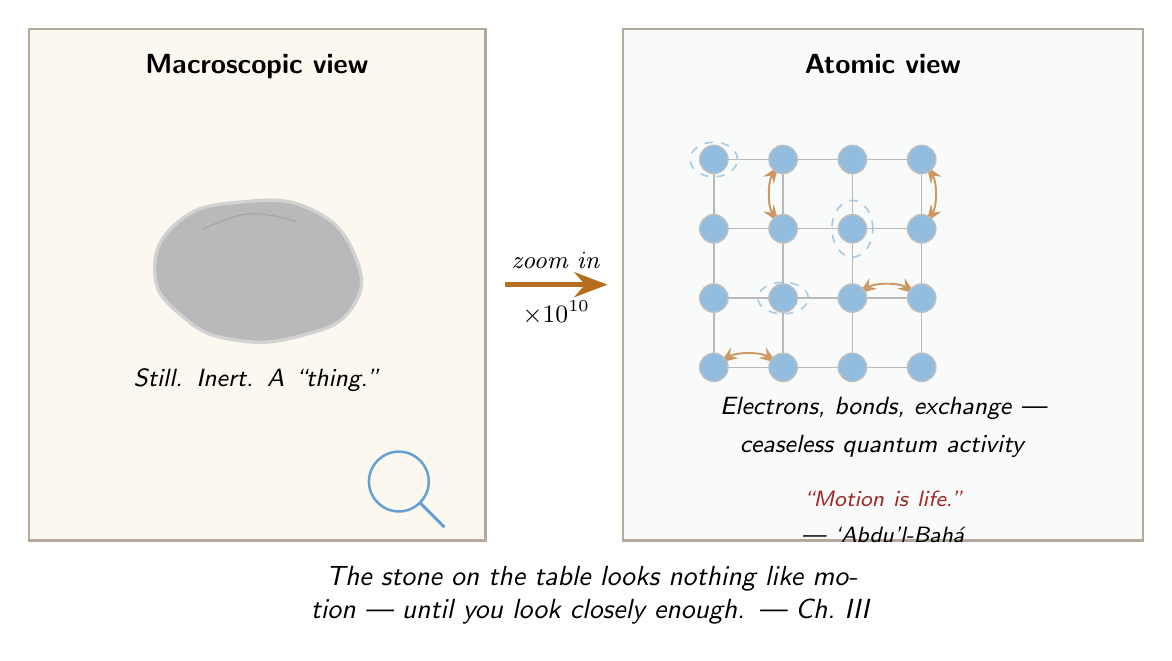
\begin{tikzpicture}[font=\sffamily]

%% ── LEFT PANEL: Macroscopic view ─────────────────────────────────────────
\begin{scope}
  % Panel background
  \fill[bgcream] (0,0) rectangle (5.8,6.5);
  \draw[panelborder, line width=0.8pt] (0,0) rectangle (5.8,6.5);

  % Panel title
  \node[anchor=north] at (2.9,6.3) {\textbf{Macroscopic view}};

  % Stone shape — smooth rounded polygon suggesting a river pebble
  \begin{scope}[shift={(2.9,3.4)}]
    \draw[fill=gray!55, draw=gray!35, very thick, line join=round]
      plot[smooth cycle, tension=0.8] coordinates {
        (-1.3, 0.0)
        (-1.0, 0.65)
        (-0.2, 0.90)
        ( 0.7, 0.80)
        ( 1.25, 0.20)
        ( 1.20,-0.45)
        ( 0.55,-0.80)
        (-0.30,-0.85)
        (-0.95,-0.55)
      };
    % Subtle highlight to give 3-D feel
    \draw[gray!80, line width=0.4pt, opacity=0.6]
      plot[smooth, tension=0.7] coordinates {
        (-0.7, 0.55) (-0.1, 0.75) (0.5, 0.65)
      };
  \end{scope}

  % Caption beneath stone
  \node[anchor=north, text width=4.8cm, align=center] at (2.9,2.3)
    {\small\textit{Still. Inert. A ``thing.''}};

  % Magnifying glass icon — bottom right corner
  \begin{scope}[shift={(4.7,0.75)}]
    \draw[atomblue, line width=0.9pt] (0,0) circle (0.38);
    \draw[atomblue, line width=1.1pt] (0.27,-0.27) -- (0.58,-0.58);
  \end{scope}
\end{scope}

%% ── ZOOM ARROW between panels ─────────────────────────────────────────────
\begin{scope}[shift={(5.8,3.25)}]
  \draw[procamber, ->, line width=2pt, >=Stealth]
    (0.25,0) -- (1.55,0);
  \node[above, font=\small] at (0.90, 0.08) {\small\textit{zoom in}};
  \node[below, font=\small] at (0.90,-0.08) {\small$\times 10^{10}$};
\end{scope}

%% ── RIGHT PANEL: Atomic view ──────────────────────────────────────────────
\begin{scope}[shift={(7.55,0)}]
  % Panel background — slightly blue-tinted
  \fill[bgcream!80!atomblue!18] (0,0) rectangle (6.6,6.5);
  \draw[panelborder, line width=0.8pt] (0,0) rectangle (6.6,6.5);

  % Panel title
  \node[anchor=north] at (3.3,6.3) {\textbf{Atomic view}};

  % ── Bond lines (drawn first, behind atoms) ──────────────────────────────
  \begin{scope}[shift={(1.15,2.20)}]
    \def\dx{0.88}  % horizontal spacing
    \def\dy{0.88}  % vertical spacing
    \def\nr{4}     % rows
    \def\nc{4}     % cols (0-indexed max = 3)

    % Horizontal bonds
    \foreach \row in {0,1,2,3}{
      \foreach \col in {0,1,2}{
        \draw[gray!55, line width=0.5pt]
          ({\col*\dx},{\row*\dy}) -- ({(\col+1)*\dx},{\row*\dy});
      }
    }
    % Vertical bonds
    \foreach \row in {0,1,2}{
      \foreach \col in {0,1,2,3}{
        \draw[gray!55, line width=0.5pt]
          ({\col*\dx},{\row*\dy}) -- ({\col*\dx},{(\row+1)*\dy});
      }
    }

    % ── Quantum exchange arrows (↔) between select atom pairs ──────────────
    \foreach \px/\py/\qx/\qy in {
        0/0/1/0,
        2/1/3/1,
        1/2/1/3,
        3/3/3/2}{
      \draw[procamber!70, <->, >=Stealth, line width=0.7pt,
            bend left=35,
            shorten <=3pt, shorten >=3pt]
        ({\px*\dx},{\py*\dy}) to ({\qx*\dx},{\qy*\dy});
    }

    % ── Electron orbital arcs around selected atoms ─────────────────────────
    % Atom at (1,1)
    \draw[atomblue!55, dashed, line width=0.6pt]
      ({\dx},{\dy}) ellipse (0.32 and 0.20);
    % Atom at (2,2)
    \draw[atomblue!55, dashed, line width=0.6pt]
      ({2*\dx},{2*\dy}) ellipse (0.26 and 0.36);
    % Atom at (0,3)
    \draw[atomblue!55, dashed, line width=0.6pt]
      (0,{3*\dy}) ellipse (0.30 and 0.22);

    % ── Atom circles (drawn on top) ─────────────────────────────────────────
    \foreach \row in {0,1,2,3}{
      \foreach \col in {0,1,2,3}{
        \draw[fill=atomblue!70, draw=gray!50, line width=0.5pt]
          ({\col*\dx},{\row*\dy}) circle (0.18);
      }
    }
  \end{scope}

  % Caption beneath grid
  \node[anchor=north, text width=6.0cm, align=center] at (3.3,1.95)
    {\small\textit{Electrons, bonds, exchange ---}\\[2pt]
     \small\textit{ceaseless quantum activity}};

  % Quote below caption — extra clearance from the 2-line caption above
  \node[anchor=north, text width=6.0cm, align=center] at (3.3,0.75)
    {\footnotesize\textcolor{emphred}{\textit{``Motion is life.''}}\\[1pt]
     \footnotesize\textit{--- \textquoteleft Abdu\textquoteright l-Bah\'a}};
\end{scope}

%% ── CAPTION below entire figure ───────────────────────────────────────────
\node[anchor=north, text width=13.5cm, align=center] at (7.15,-0.20)
  {\textit{The stone on the table looks nothing like motion --- until you look closely enough. --- Ch.~III}};

\end{tikzpicture}
\end{document}
